\documentclass{article}
\usepackage{ctex}
\usepackage[a4paper,left=10mm,right=10mm,top=15mm,bottom=15mm]{geometry}
\usepackage{graphicx}
\usepackage{amsfonts,amssymb}
\usepackage{amsmath}
\usepackage{biblatex}
\usepackage{hyperref}
\usepackage{color}
\usepackage{titlesec}
\usepackage{titletoc}

\title{VI-SLAM系统初始化闭式可解性分析}
\author{张谦}
\date{\today}
\begin{document}
\maketitle
\tableofcontents
\newpage

\section{系统模型}
由VI-SLAM系统可观性分析可知,在给定视觉和IMU观测后,body系的全局平移和重力方向旋转yaw角不可观,
body系的速度、重力和绝对尺度是可观的。分析VI-SLAM系统初始化时的闭式可解性,亦即分析在一段时间内,
在不同条件下可观变量的可解性:(1)运动轨迹和状态;(2)地图点数量和观测图像上的分布;(3)相机图像帧数。
\par
为简化分析,不考虑相机和IMU之间的外参,即假设相机和IMU位姿重合。在该系统中,四元数表示旋转采用Hamilton形式。坐标系约定:全局坐标系用$G$表示,Camera坐标系用$C$表示,
IMU坐标系用$I$表示,地图点用$f$表示;相机、IMU和地图点表示在某个坐标系下,则该坐标系符号写在对应变量符号的左上角,
变量标识写在变量符号的右下角,例如$\sideset{^G}{}{\mathop{\mathbf{p}_{I}}}$表示IMU系(body系)原点在全局坐标系中的位置(平移),
$\sideset{^G}{}{\mathop{\textbf{v}_{I}}}$表示IMU系在全局坐标系下的速度,$\sideset{^G}{}{\mathop{\textbf{q}_{I}}}$表示从全局坐标系
旋转到IMU系的单位四元数,由于采用Hamilton形式,旋转均是由$I$系到$G$系旋转,与JPL表示方式相反;$\sideset{^G}{}{\mathop{\textbf{p}_{f_i}}}$
表示第$i$个地图点在$G$系下的坐标。
\begin{figure}[ht]
    \centering
    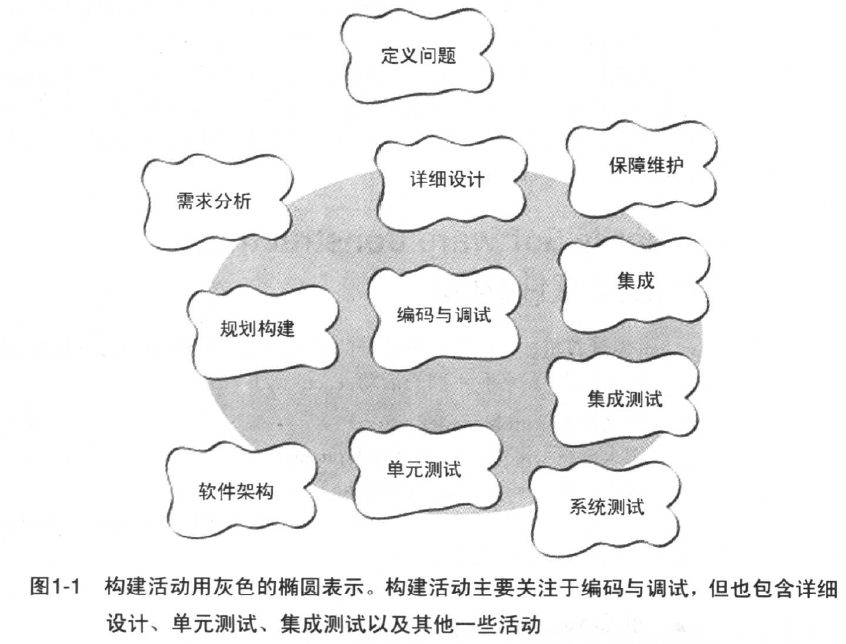
\includegraphics[width=15cm]{figure1.png}
    \caption{几何关系}
    \label{figs:geometryRelation}
\end{figure}

\par
陀螺仪测量$\sideset{^I}{}{\mathop{\mathbf{\omega}_m}}$和加速度计测量$\sideset{^I}{}{\mathop{\mathbf{a}_m}}$模型为:
\begin{equation}
    \sideset{^I}{}{\mathop{\mathbf{\omega}_{m}(t)}}=\sideset{^I}{}{\mathop{\mathbf{\omega}(t)}}
    +\textbf{b}_{g}(t)+\textbf{n}_{g}(t)
\end{equation}
\begin{equation}
    \sideset{^I}{}{\mathop{\mathbf{a}_{m}(t)}}=\textbf{C}^T(\sideset{^G}{}{\mathop{\mathbf{q}_{I}(t)}})
    (\sideset{^G}{}{\mathop{\mathbf{a}_{I}(t)}}-\sideset{^G}{}{\mathop{\mathbf{g}}})
    +\textbf{b}_{a}(t)+\textbf{n}_{a}(t)
\end{equation}
其中$\textbf{C}(\mathbf{q})$表示四元数对应的旋转矩阵。在分析可解性时,若不考虑噪声影响,则有,
\begin{equation}
    \sideset{^I}{}{\mathop{\mathbf{\omega}_{m}(t)}}=\sideset{^I}{}{\mathop{\mathbf{\omega}(t)}}
    +\textbf{b}_{g}(t)
\end{equation}
\begin{equation}
    \sideset{^G}{}{\mathop{\mathbf{a}_{I}(t)}}=\textbf{C}(\sideset{^G}{}{\mathop{\mathbf{q}_{I}(t)}})
    (\sideset{^I}{}{\mathop{\mathbf{a}_{m}(t)}}-\textbf{b}_{a}(t))
    +\sideset{^G}{}{\mathop{\mathbf{g}}}
\end{equation}

\par
现分析时间段$\left[t_{in},t_{fin}\right]$内的可解性,如图\ref{figs:geometryRelation}所示,
从$t_{in}$到$t\in\left[t_{in},t_{fin}\right]$时刻的平移几何关系可表示为,
\begin{equation}
    \begin{array}{ll}
        \sideset{^G}{}{\mathop{\textbf{p}_{I}}}(t)&=\sideset{^G}{}{\mathop{\textbf{p}_{I}}}(t_{in})+
        \sideset{^G}{}{\mathop{\textbf{v}_{I}}}(t_{in})\Delta{t}+\iint_{t_{in}}^{t}\sideset{^G}{}{\mathop{\mathbf{a}_{I}(\tau)}}d{\tau}^2\\
        &=\sideset{^G}{}{\mathop{\textbf{p}_{I}}}(t_{in})+
        \sideset{^G}{}{\mathop{\textbf{v}_{I}}}(t_{in})\Delta{t}+\iint_{t_{in}}^{t}
        (\textbf{C}(\sideset{^G}{}{\mathop{\mathbf{q}_{I}(\tau)}})(
        \sideset{^I}{}{\mathop{\mathbf{a}_{m}(\tau)}}-\textbf{b}_{a}(\tau))
        +\sideset{^G}{}{\mathop{\mathbf{g}}})d{\tau}^2\\
        &=\sideset{^G}{}{\mathop{\textbf{p}_{I}}}(t_{in})+
        \sideset{^G}{}{\mathop{\textbf{v}_{I}}}(t_{in})\Delta{t}
        +\frac{1}{2}\sideset{^G}{}{\mathop{\mathbf{g}}}\Delta{t}^{2}
        +\iint_{t_{in}}^{t}\textbf{C}(\sideset{^G}{}{\mathop{\mathbf{q}_{I}(\tau)}})
        (\sideset{^I}{}{\mathop{\mathbf{a}_{m}(\tau)}}-\textbf{b}_{a}(\tau))d{\tau}^2\\
        &=\sideset{^G}{}{\mathop{\textbf{p}_{I}}}(t_{in})+
        \sideset{^G}{}{\mathop{\textbf{v}_{I}}}(t_{in})\Delta{t}
        +\frac{1}{2}\sideset{^G}{}{\mathop{\mathbf{g}}}\Delta{t}^{2}
        +\textbf{C}(\sideset{^G}{}{\mathop{\mathbf{q}_{I}(t_{in})}})\textbf{C}^T(\sideset{^G}{}{\mathop{\mathbf{q}_{I}(t_{in})}})
        \iint_{t_{in}}^{t}\textbf{C}(\sideset{^G}{}{\mathop{\mathbf{q}_{I}(\tau)}})
        (\sideset{^I}{}{\mathop{\mathbf{a}_{m}(\tau)}}-\textbf{b}_{a}(\tau))d{\tau}^2\\
        &=\sideset{^G}{}{\mathop{\textbf{p}_{I}}}(t_{in})+
        \sideset{^G}{}{\mathop{\textbf{v}_{I}}}(t_{in})\Delta{t}
        +\frac{1}{2}\sideset{^G}{}{\mathop{\mathbf{g}}}\Delta{t}^{2}
        +\textbf{C}(\sideset{^G}{}{\mathop{\mathbf{q}_{I}(t_{in})}})
        \iint_{t_{in}}^{t}\textbf{C}^T(\sideset{^G}{}{\mathop{\mathbf{q}_{I}(t_{in})}})\textbf{C}(\sideset{^G}{}{\mathop{\mathbf{q}_{I}(\tau)}})
        (\sideset{^I}{}{\mathop{\mathbf{a}_{m}(\tau)}}-\textbf{b}_{a}(\tau))d{\tau}^2\\
        &=\sideset{^G}{}{\mathop{\textbf{p}_{I}}}(t_{in})+
        \sideset{^G}{}{\mathop{\textbf{v}_{I}}}(t_{in})\Delta{t}
        +\frac{1}{2}\sideset{^G}{}{\mathop{\mathbf{g}}}\Delta{t}^{2}
        +\textbf{C}(\sideset{^G}{}{\mathop{\mathbf{q}_{I}(t_{in})}})
        \iint_{t_{in}}^{t}\textbf{C}(\sideset{^{I_{in}}}{}{\mathop{\mathbf{q}_{I}(\tau)}})
        (\sideset{^I}{}{\mathop{\mathbf{a}_{m}(\tau)}}-\textbf{b}_{a}(\tau))d{\tau}^2\\
        &=\sideset{^G}{}{\mathop{\textbf{p}_{I}}}(t_{in})+
        \sideset{^G}{}{\mathop{\textbf{v}_{I}}}(t_{in})\Delta{t}
        +\frac{1}{2}\sideset{^G}{}{\mathop{\mathbf{g}}}\Delta{t}^{2}\\
        &\hspace{1cm}+\textbf{C}(\sideset{^G}{}{\mathop{\mathbf{q}_{I}(t_{in})}})
        (\iint_{t_{in}}^{t}\textbf{C}(\sideset{^{I_{in}}}{}{\mathop{\mathbf{q}_{I}(\tau)}})
        \sideset{^I}{}{\mathop{\mathbf{a}_{m}(\tau)}}d{\tau}^2
        -\iint_{t_{in}}^{t}\textbf{C}(\sideset{^{I_{in}}}{}{\mathop{\mathbf{q}_{I}(\tau)}})
        \textbf{b}_{a}(\tau)d{\tau}^2)
    \end{array}
\end{equation}
假设在积分区间内,加速度计bias为常量,则有,
\begin{equation}\label{eqs:imuInG}
    \begin{array}{ll}
        \sideset{^G}{}{\mathop{\textbf{p}_{I}}}(t)
        &=\sideset{^G}{}{\mathop{\textbf{p}_{I}}}(t_{in})+
        \sideset{^G}{}{\mathop{\textbf{v}_{I}}}(t_{in})\Delta{t}
        +\frac{1}{2}\sideset{^G}{}{\mathop{\mathbf{g}}}\Delta{t}^{2}\\
        &\hspace{1cm}+\textbf{C}(\sideset{^G}{}{\mathop{\mathbf{q}_{I}(t_{in})}})
        (\iint_{t_{in}}^{t}\textbf{C}(\sideset{^{I_{in}}}{}{\mathop{\mathbf{q}_{I}(\tau)}})
        \sideset{^I}{}{\mathop{\mathbf{a}_{m}(\tau)}}d{\tau}^2
        -\iint_{t_{in}}^{t}\textbf{C}(\sideset{^{I_{in}}}{}{\mathop{\mathbf{q}_{I}(\tau)}})
        d{\tau}^2\textbf{B})\\
        &=\sideset{^G}{}{\mathop{\textbf{p}_{I}}}(t_{in})+
        \sideset{^G}{}{\mathop{\textbf{v}_{I}}}(t_{in})\Delta{t}
        +\frac{1}{2}\sideset{^G}{}{\mathop{\mathbf{g}}}\Delta{t}^{2}
        +\textbf{C}(\sideset{^G}{}{\mathop{\mathbf{q}_{I}(t_{in})}})
        (\sideset{^{I_{in}}}{}{\mathop{\textbf{S}_{I}(t)}}
        -\sideset{^{I_{in}}}{}{\mathop{{\Gamma}_{I}(t)}}\textbf{B})
    \end{array}
\end{equation}
其中
\begin{equation}
    \sideset{^{I_{in}}}{}{\mathop{\textbf{S}_{I}(t)}}=\iint_{t_{in}}^{t}\textbf{C}(\sideset{^{I_{in}}}{}{\mathop{\mathbf{q}_{I}(\tau)}})
    \sideset{^I}{}{\mathop{\mathbf{a}_{m}(\tau)}}d{\tau}^2
\end{equation}
\begin{equation}
    \sideset{^{I_{in}}}{}{\mathop{{\Gamma}_{I}(t)}}=\iint_{t_{in}}^{t}\textbf{C}(\sideset{^{I_{in}}}{}{\mathop{\mathbf{q}_{I}(\tau)}})
    d{\tau}^2
\end{equation}
且$\sideset{^{I_{in}}}{}{\mathop{\textbf{S}_{I}(t)}}$和$\sideset{^{I_{in}}}{}{\mathop{{\Gamma}_{I}(t)}}$可由加速度计和陀螺仪提供的测量积分得到。

\par
先假设有N个地图点被同时观测到,$\sideset{^G}{}{\mathop{\textbf{p}_{f_i}}},i=1,\dots,N$,表示在第$t$时刻的相机
坐标系下为$\sideset{^{I_t}}{}{\mathop{\textbf{p}_{f_i}}}$,则有,
\begin{equation}\label{eqs:mappointInG1}
    \sideset{^G}{}{\mathop{\textbf{p}_{f_i}}}=\sideset{^G}{}{\mathop{\textbf{p}_I}}(t)
    +\textbf{C}(\sideset{^G}{}{\mathop{\textbf{q}_{I}}}(t_{in}))\textbf{C}(\sideset{^{I_{in}}}{}{\mathop{\textbf{q}_{I}}}(t))
    \sideset{^{I_t}}{}{\mathop{\textbf{p}_{f_i}}}
\end{equation}
若上式中$t=t_{in}$,则有,
\begin{equation}\label{eqs:mappointInG2}
    \sideset{^G}{}{\mathop{\textbf{p}_{f_i}}}=\sideset{^G}{}{\mathop{\textbf{p}_I}}(t_{in})
    +\textbf{C}(\sideset{^G}{}{\mathop{\textbf{q}_{I}}}(t_{in}))
    \sideset{^{I_{in}}}{}{\mathop{\textbf{p}_{f_i}}}
\end{equation}
将(\ref{eqs:imuInG})和(\ref{eqs:mappointInG2})带入(\ref{eqs:mappointInG1}),得到,
\begin{equation}
    \begin{array}{ll}
        \sideset{^G}{}{\mathop{\textbf{p}_I}}(t_{in})
        +\textbf{C}(\sideset{^G}{}{\mathop{\textbf{q}_{I}}}(t_{in}))
        \sideset{^{I_{in}}}{}{\mathop{\textbf{p}_{f_i}}}
        &=\sideset{^G}{}{\mathop{\textbf{p}_{I}}}(t_{in})+
        \sideset{^G}{}{\mathop{\textbf{v}_{I}}}(t_{in})\Delta{t}
        +\frac{1}{2}\sideset{^G}{}{\mathop{\mathbf{g}}}\Delta{t}^{2}
        +\textbf{C}(\sideset{^G}{}{\mathop{\mathbf{q}_{I}(t_{in})}})
        (\sideset{^{I_{in}}}{}{\mathop{\textbf{S}_{I}(t)}}
        -\sideset{^{I_{in}}}{}{\mathop{{\Gamma}_{I}(t)}}\textbf{B})\\
        &\hspace{1cm}+\textbf{C}(\sideset{^G}{}{\mathop{\textbf{q}_{I}}}(t_{in}))\textbf{C}(\sideset{^{I_{in}}}{}{\mathop{\textbf{q}_{I}}}(t))
        \sideset{^{I_t}}{}{\mathop{\textbf{p}_{f_i}}}\\
        \Leftrightarrow
        \textbf{C}(\sideset{^G}{}{\mathop{\textbf{q}_{I}}}(t_{in}))
        \sideset{^{I_{in}}}{}{\mathop{\textbf{p}_{f_i}}}
        &=\sideset{^G}{}{\mathop{\textbf{v}_{I}}}(t_{in})\Delta{t}
        +\frac{1}{2}\sideset{^G}{}{\mathop{\mathbf{g}}}\Delta{t}^{2}
        +\textbf{C}(\sideset{^G}{}{\mathop{\mathbf{q}_{I}(t_{in})}})
        (\sideset{^{I_{in}}}{}{\mathop{\textbf{S}_{I}(t)}}
        -\sideset{^{I_{in}}}{}{\mathop{{\Gamma}_{I}(t)}}\textbf{B})\\
        &\hspace{1cm}+\textbf{C}(\sideset{^G}{}{\mathop{\textbf{q}_{I}}}(t_{in}))\textbf{C}(\sideset{^{I_{in}}}{}{\mathop{\textbf{q}_{I}}}(t))
        \sideset{^{I_t}}{}{\mathop{\textbf{p}_{f_i}}}
    \end{array}
\end{equation}
两边同时乘以$\textbf{C}^T(\sideset{^G}{}{\mathop{\textbf{q}_{I}}}(t_{in}))$,得到,
\begin{equation}\label{eqs:geometryRelation1}
    \begin{array}{ll}
        &\sideset{^{I_{in}}}{}{\mathop{\textbf{p}_{f_i}}}
        =\textbf{C}^T(\sideset{^G}{}{\mathop{\textbf{q}_{I}}}(t_{in}))
        (\sideset{^G}{}{\mathop{\textbf{v}_{I}}}(t_{in})\Delta{t}
        +\frac{1}{2}\sideset{^G}{}{\mathop{\mathbf{g}}}\Delta{t}^{2}
        +\textbf{C}(\sideset{^G}{}{\mathop{\mathbf{q}_{I}(t_{in})}})
        (\sideset{^{I_{in}}}{}{\mathop{\textbf{S}_{I}(t)}}
        -\sideset{^{I_{in}}}{}{\mathop{{\Gamma}_{I}(t)}}\textbf{B}))
        +\textbf{C}(\sideset{^{I_{in}}}{}{\mathop{\textbf{q}_{I}}}(t))
        \sideset{^{I_t}}{}{\mathop{\textbf{p}_{f_i}}}\\
        &\Leftrightarrow
        \textbf{C}(\sideset{^{I_{in}}}{}{\mathop{\textbf{q}_{I}}}(t))
        \sideset{^{I_t}}{}{\mathop{\textbf{p}_{f_i}}}
        =\sideset{^{I_{in}}}{}{\mathop{\textbf{p}_{f_i}}}
        -\sideset{^{I_{in}}}{}{\mathop{\textbf{v}_I}}\Delta{t}
        -\frac{1}{2}\sideset{^{I_{in}}}{}{\mathop{\mathbf{g}}}\Delta{t}^{2}
        -\sideset{^{I_{in}}}{}{\mathop{\textbf{S}_{I}(t)}}
        +\sideset{^{I_{in}}}{}{\mathop{{\Gamma}_{I}(t)}}\textbf{B}
    \end{array}
\end{equation}
其中
\begin{equation}
    \sideset{^{I_{in}}}{}{\mathop{\textbf{v}_I}}
    =\textbf{C}^T(\sideset{^G}{}{\mathop{\textbf{q}_{I}}}(t_{in}))
    \sideset{^G}{}{\mathop{\textbf{v}_{I}}}(t_{in})
\end{equation}
\begin{equation}
    \sideset{^{I_{in}}}{}{\mathop{\mathbf{g}}}
    =\textbf{C}^T(\sideset{^G}{}{\mathop{\textbf{q}_{I}}}(t_{in}))
    \sideset{^G}{}{\mathop{\mathbf{g}}}
\end{equation}

\par
假设在时间段$t_{in},t_{fin}$内,共有$M$帧图像:$t_1=t_{in}<t_2<\dots<t_M=t_{fin}$,且$N$个地图点
均被这M帧图像观测到。为简化书写,利用如下简写:
\begin{equation}
    \begin{array}{ll}
        &\textbf{P}_j^i\triangleq\textbf{C}(\sideset{^{I_{in}}}{}{\mathop{\textbf{q}_{I}}}(t_j))
        \sideset{^{I_{t_j}}}{}{\mathop{\textbf{p}_{f_i}}}\\
        &\textbf{P}^i \triangleq \sideset{^{I_{in}}}{}{\mathop{\textbf{p}_{f_i}}}\\
        &\textbf{V} \triangleq \sideset{^{I_{in}}}{}{\mathop{\textbf{v}_I}}\\
        &\textbf{G} \triangleq \sideset{^{I_{in}}}{}{\mathop{\mathbf{g}}}\\
        &\Gamma_j \triangleq \sideset{^{I_{in}}}{}{\mathop{{\Gamma}_{I}(t_j)}}\\
        &\textbf{S}_j \triangleq \sideset{^{I_{in}}}{}{\mathop{\textbf{S}_{I}(t_j)}}
    \end{array}
\end{equation}
其中$i=1,2,\dots,N;\ \ j=1,2,\dots,M$。另外,用$\mathbf{\mu}_j^i$表示$\textbf{P}_j^i$的单位向量,
则有$\textbf{P}_j^i=\lambda_j^i\mathbf{\mu}_j^i$。不失一般性,可令$t_{in}=0$,则有$\Delta{t}=t$。
几何关系式(\ref{eqs:geometryRelation1})在每个图像帧时刻$t_j$,可表示为
\begin{equation}\label{eqs:geometryRelation2}
    \textbf{P}^i-\textbf{V}t_j-\frac{1}{2}\textbf{G}t_j^2+\Gamma_j\textbf{B}
    -\lambda_j^i\mathbf{\mu}_j^i=\textbf{S}_j
\end{equation}
另外当$j=1$时,$t_j=t_1=t_{in}=0$,则有$\textbf{P}^i=\textbf{P}^i_1=\lambda_1^i\mathbf{\mu}_1^i$。
几何关系(\ref{eqs:geometryRelation2})可进一步表示为,
\begin{equation}\label{eqs:geometryRelation3}
    -\textbf{V}t_j-\frac{1}{2}\textbf{G}t_j^2+\Gamma_j\textbf{B}+\lambda_1^i\mathbf{\mu}_1^i
    -\lambda_j^i\mathbf{\mu}_j^i=\textbf{S}_j
\end{equation}
对于第$t_1$帧和第$t_j$帧,第1个地图点和第$i$个地图点,有如下几何关系:
\begin{equation}\label{eqs:geometryRelation4}
    \lambda_1^1\mathbf{\mu}_1^1-\lambda_j^1\mathbf{\mu}_j^1
    =\lambda_1^i\mathbf{\mu}_1^i-\lambda_j^i\mathbf{\mu}_j^i
\end{equation}
综合几何关系(\ref{eqs:geometryRelation3})和(\ref{eqs:geometryRelation4}),可最终得到如下关系式子,
\begin{equation}\label{eqs:geometryRelation5}
    \left\{\begin{array}{c}
        -\textbf{V}t_j-\frac{1}{2}\textbf{G}t_j^2+\Gamma_j\textbf{B}+\lambda_1^1\mathbf{\mu}_1^1
        -\lambda_j^1\mathbf{\mu}_j^1=\textbf{S}_j\\
        \lambda_1^1\mathbf{\mu}_1^1-\lambda_j^1\mathbf{\mu}_j^1
        -\lambda_1^i\mathbf{\mu}_1^i+\lambda_j^i\mathbf{\mu}_j^i=\textbf{0}_3
    \end{array}\right.
\end{equation}
其中$j=2,3,\dots,M;\ \ i=2,3,\dots,N$。
分析VI-SLAM系统初始化的闭式可解性,亦即分析在几何关系(\ref{eqs:geometryRelation5})下,
变量$\textbf{P}^i_j,\textbf{V},\textbf{G},\textbf{B}$的可解性。其中(\ref{eqs:geometryRelation5})
可提供$3*(M-1)*N$个方程,未知变量有$M*N+6$维(不考虑bias)或$M*N+9$维(只考虑加速度计bias)。
\par
定义如下变量和矩阵:
考虑加速度计bias未知变量,
\begin{equation}
    \textbf{X}\triangleq\left[\textbf{G}^T,\textbf{V}^T,\textbf{B}^T,\lambda_1^1,\dots,\lambda_1^N,
    \dots,\lambda_M^1,\dots,\lambda_M^N\right]^T
\end{equation}
不考虑bias未知变量,
\begin{equation}
    \textbf{X}\triangleq\left[\textbf{G}^T,\textbf{V}^T,\lambda_1^1,\dots,\lambda_1^N,
    \dots,\lambda_M^1,\dots,\lambda_M^N\right]^T
\end{equation}
IMU测量相关积分变量,
\begin{equation}
    \textbf{S}\triangleq \left[\textbf{S}_2^T,\textbf{0}_{1\times3},\dots,\textbf{0}_{1\times 3},
    \textbf{S}_3^T,\textbf{0}_{1\times3},\dots,\textbf{0}_{1\times 3},
    \textbf{S}_M^T,\textbf{0}_{1\times3},\dots,\textbf{0}_{1\times 3}\right]^T
\end{equation}
几何关系矩阵,
\begin{equation}
    \Xi=\left[\begin{array}{cccccccccccccc}
        \textbf{T}_2&\textbf{K}_2&\Gamma_2&\mathbf{\mu}_1^1&\textbf{0}_{3\times 1}&\dots&\textbf{0}_{3\times 1}&
        -\mathbf{\mu}_2^1&\textbf{0}_{3\times 1}&\dots&\textbf{0}_{3\times 1}&\dots&\dots&\textbf{0}_{3\times 1}\\
        \textbf{0}_{3\times 3}&\textbf{0}_{3\times 3}&\textbf{0}_{3\times 3}&\mathbf{\mu}_1^1&-\mathbf{\mu}_1^2&\dots&\textbf{0}_{3\times 1}&
        -\mathbf{\mu}_2^1&\mathbf{\mu}_2^2&\dots&\textbf{0}_{3\times 1}&\dots&\dots&\textbf{0}_{3\times 1}\\
        \dots&\dots&\dots&\dots&\dots&\dots&\dots&\dots&\dots&\dots&\dots&\dots&\dots&\dots\\
        \textbf{0}_{3\times 3}&\textbf{0}_{3\times 3}&\textbf{0}_{3\times 3}&\mathbf{\mu}_1^1&\textbf{0}_{3\times 1}&\dots&-\mathbf{\mu}_1^N&
        -\mathbf{\mu}_2^1&\textbf{0}_{3\times 1}&\dots&\mathbf{\mu}_2^N&\dots&\dots&\textbf{0}_{3\times 1}\\
        \dots&\dots&\dots&\dots&\dots&\dots&\dots&\dots&\dots&\dots&\dots&\dots&\dots&\dots\\
        \dots&\dots&\dots&\dots&\dots&\dots&\dots&\dots&\dots&\dots&\dots&\dots&\dots&\dots\\
        \textbf{T}_M&\textbf{K}_M&\Gamma_M&\mathbf{\mu}_1^1&\textbf{0}_{3\times 1}&\dots&\dots&
        \dots&\dots&\dots&\textbf{0}_{3\times 1}&-\mathbf{\mu}_M^1&\dots&\textbf{0}_{3\times 1}\\
        \textbf{0}_{3\times 3}&\textbf{0}_{3\times 3}&\textbf{0}_{3\times 3}&\mathbf{\mu}_1^1&-\mathbf{\mu}_1^2&\dots&\dots&
        \dots&\dots&\dots&\textbf{0}_{3\times 1}&-\mathbf{\mu}_M^1&\mathbf{\mu}_M^2&\textbf{0}_{3\times 1}\\
        \dots&\dots&\dots&\dots&\dots&\dots&\dots&\dots&\dots&\dots&\dots&\dots&\dots&\dots\\
        \textbf{0}_{3\times 3}&\textbf{0}_{3\times 3}&\textbf{0}_{3\times 3}&\mathbf{\mu}_1^1&\textbf{0}_{3\times 1}&\dots&-\mathbf{\mu}_1^N&
        \textbf{0}_{3\times 1}&\dots&\dots&\textbf{0}_{3\times 1}&-\mathbf{\mu}_M^1&\dots&\mathbf{\mu}_M^N
    \end{array}\right]
\end{equation}
其中$\textbf{T}_j\triangleq -\frac{t_j^2}{2}\textbf{I}_3$和$\textbf{K}_j\triangleq -t_j\textbf{I}_3$。

\par
根据以上定义,对于M帧图像和N个地图点的几何关系式(\ref{eqs:geometryRelation5})可表示为
\begin{equation}\label{eqs:geometryRelation6}
    \Xi\textbf{X}=\textbf{S}
\end{equation}
假设重力的大小已知,即$|\textbf{G}|=g$,则对方程组(\ref{eqs:geometryRelation6})添加如下约束,
\begin{equation}\label{eqs:geometryRelation7}
    |\Pi\textbf{X}|^2=g^2
\end{equation}
其中$\Pi\triangleq \left[\textbf{I}_3,\textbf{0}_3,\dots,\textbf{0}_3\right]$。

\par
至此,VI-SLAM系统初始化的闭式可解性分析,将基于方程组(\ref{eqs:geometryRelation6})和(\ref{eqs:geometryRelation7})。


\section{闭式解方程}

\section{可解性分析:Unbiased Case}
\subsection{Planar Case}

\subsection{Linear Case}

\subsection{图像帧数小于等于2}

\subsection{图像帧数等于3}

\subsection{图像帧数大于等于4}

\subsection{Constant Acceleration}

\section{可解性分析:Biased Case}
\subsection{图像帧数小于等于3}

\subsection{图像帧数等于4}

\subsection{图像帧数大于等于5}

\section{Gyroscope Bias估计}

\section{Modified MK闭式解}


\begin{thebibliography}{99}  
    \bibitem{zhihu}https://www.zhihu.com/question/22983179
    \bibitem{Meyer2000}Meyer CD (2000) Matrix Analysis and Applied Linear Algebra. Philadelphia, PA: SIAM.
    \bibitem{consistency} Hesch J A, Kottas D G, Bowman S L, et al. Camera-IMU-based localization: Observability analysis and consistency improvement[J]. The International Journal of Robotics Research, 2014, 33(1): 182-201.
    \bibitem{rvio} Huai Z, Huang G. Robocentric visual-inertial odometry[C]//2018 IEEE/RSJ International Conference on Intelligent Robots and Systems (IROS). IEEE, 2018: 6319-6326.
\end{thebibliography}



\end{document}

